\section{Version Control, Git, and GitHub}
Version control is a critically important habit to develop early on.
In the simplest form, version control provides a means of keeping track of the changes you've made to your code as you go, as well as providing information about who made which changes in a collaborative project.
More complicated version control can lead to things like software written for different types of hardware, or for different scales of calculations, etc.
Many of us have used version control at some point in our educations, whether we realized it or not.
How many times have you had a document labelled "Document\_v2\_Final\_FINAL\_FINAL\_v3"?
That is an example (albeit not the greatest) of version control.
Keeping track of changes made and versions of your code can be a way to safeguard your work against potential losses and help you track down the source of bugs and errors that may arise.


The most commonly used tool for version control is \texttt{git}, with related websites \href{https://www.github.com}{GitHub}, \href{https://about.gitlab.com/}{GitLab}, and \href{https://bitbucket.org/}{Bitbucket}. 
For the purposes of this workshop, we'll focus on using GitHub because it's free and most (if not all) of us already have accounts there.

There are a few steps to do first if you've never used \texttt{git} on your current computer before. 
These will configure your computer for use with your GitHub account. 
If you use multiple computers (including working from a HPC/Supercomputer), these steps will need to be completed for each computer you use.

\begin{center}\rule{0.5\linewidth}{0.5pt}\end{center}

Configure your local machine with an SSH-key. 
This will allow your computer to connect to other \textbf{trusted} computers that you've previously designated as such, and this includes your Github account.

\begin{Shaded}
\begin{Highlighting}[]
    \BuiltInTok{cd} \VariableTok{\$HOME}
    \FunctionTok{ssh{-}keygen}
\end{Highlighting}
\end{Shaded}

will give the following response/prompt:

\begin{verbatim}
    Generating public/private rsa key pair
    Enter file in which to save the key (/home/username/.ssh/id_rsa): 
\end{verbatim}

If the file already exists, choose a new filename such as
\texttt{git\_rsa} or something you'll recognize.

\begin{verbatim}
    Enter passphrase (empty for no passphrase): 
    Enter same passphrase again: 
\end{verbatim}

You can set a passphrase if you want, but keep in mind you'll be
entering it every single time you upload changes of your code to GitHub.
Some people choose not to have a passphrase for this particular aspect
of their work, others do.

\begin{verbatim}
    Your identification has been saved in /home/username/.ssh/git_rsa
    Your public key has been saved in /home/username/.ssh/git_rsa.pub
    The key fingerprint is:
    SHA256:8U9t+r+SwCi8Xe8uu3HCjbHa7WU51A9pArzm9+F+esk username@Computer
    The key's randomart image is:
    +---[RSA 3072]----+
    |                 |
    |       .         |
    |        +  . +   |
    |         =. =. ..|
    |      . S =*o.=..|
    |       = .oBo+..o|
    |        ..o+*o.*.|
    |       . o.+o*D .|
    |           +@Bo*o|
    +----[SHA256]-----+
\end{verbatim}
\begin{center}\rule{0.5\linewidth}{0.5pt}\end{center}
Add the SSH key to your GitHub Account to allow your computer to access
it.

Go to your account settings page and click on
\texttt{SSH\ and\ GPG\ keys}, then click on \texttt{New\ SSH\ key}.

\begin{figure}
\centering

\includegraphics[width=0.8\textwidth]{Images/GH_01.png}
\caption{GitHub Step 1}
\end{figure}
\FloatBarrier

\begin{figure}
\centering
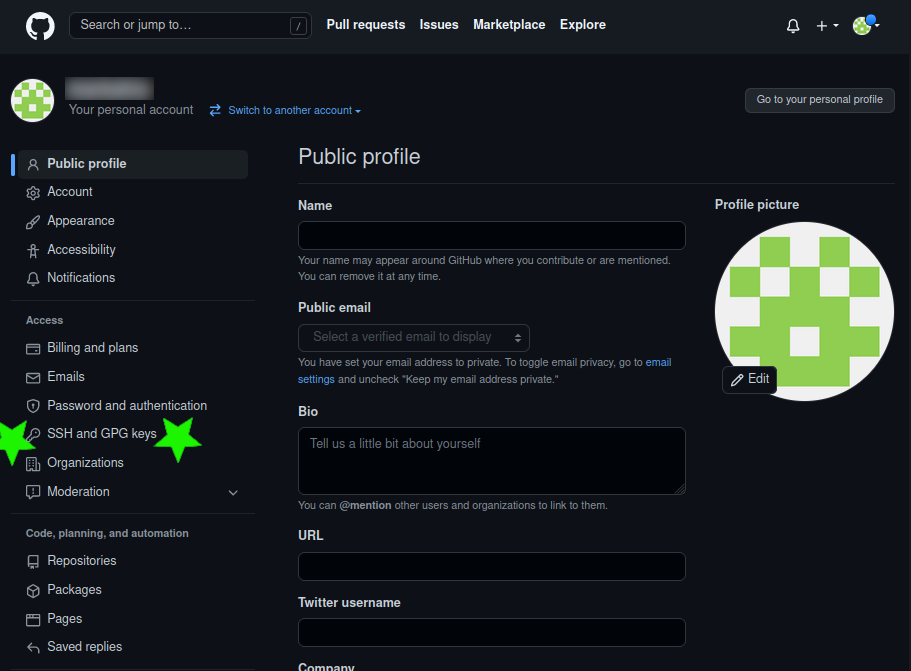
\includegraphics[width=0.8\textwidth]{Images/GH_02.png}
\caption{GitHub Step 2}
\end{figure}
\FloatBarrier

\begin{figure}
\centering
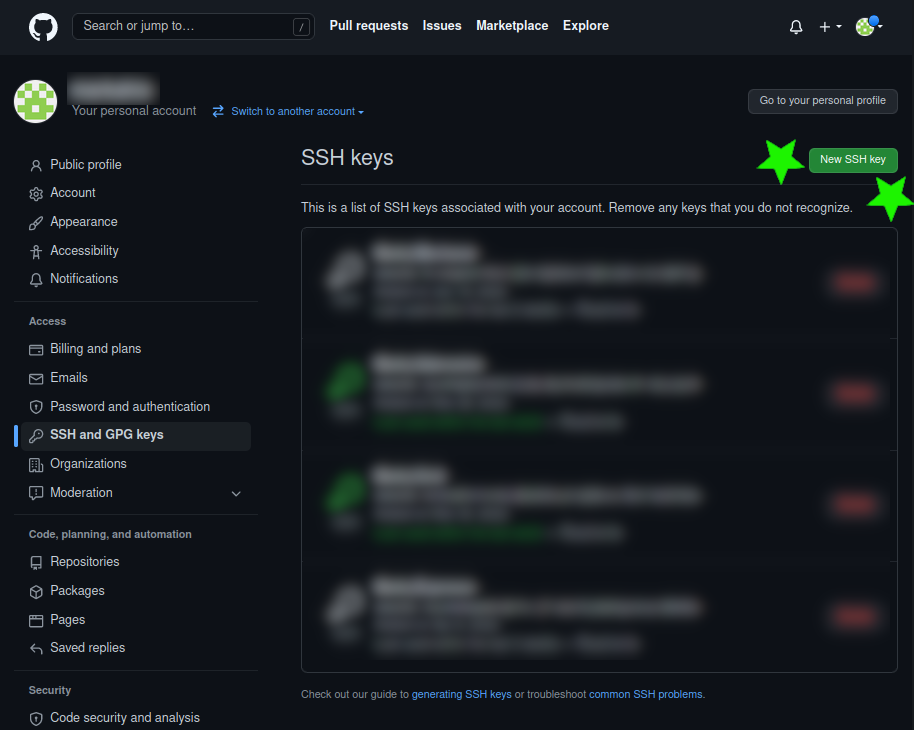
\includegraphics[width=0.8\textwidth]{Images/GH_03.png}
\caption{GitHub Step 3}
\end{figure}
\FloatBarrier

You'll need some text out of a file generated by the \texttt{ssh-keygen}
step. If you named the keyfile \texttt{git\_rsa}, the process will have
also produced a file called \texttt{git\_rsa.pub}, which is the ``public
key'' corresponding to your computer's private key. In simpler terms,
the public key is like a ``secret question'' that the other computer can
ask, that only your computer with its private ``secret answer'' can
properly respond to, so both computers know the other is trusted with
this information transfer.

Open the \texttt{git\_rsa.pub} file and copy all the text into the field
shown on the GitHub website here.

\begin{figure}
\centering
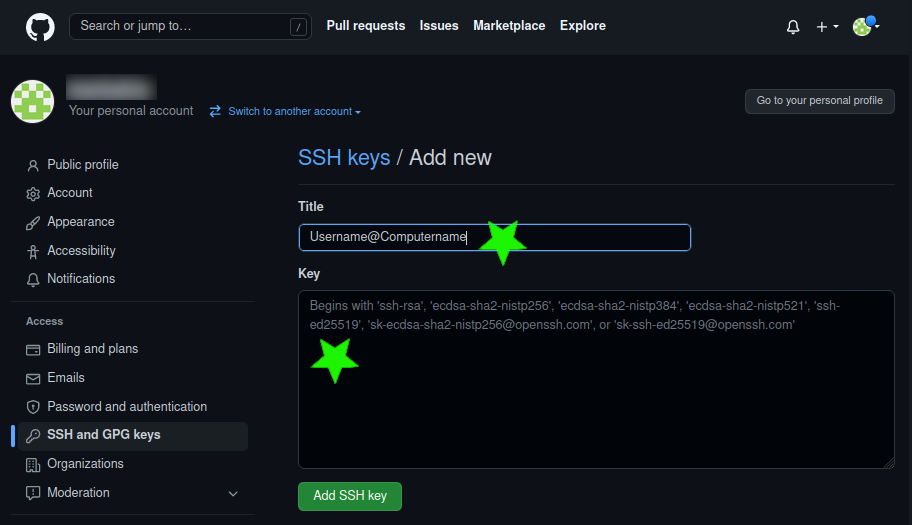
\includegraphics{Images/GH_04.png}
\caption{GitHub Step 4}
\end{figure}
\FloatBarrier

\begin{center}\rule{0.5\linewidth}{0.5pt}\end{center}

You'll also need to configure \texttt{git} on your computer as well.
Assuming you have \texttt{git} already installed, you can begin with
setting some of the initial variables.

You can configure individual repositories (projects) with these
settings, or you can configure \texttt{git} globally to set your
defaults. For now, we'll assume that you only have one GitHub account to
manage on your computer.

\begin{Shaded}
\begin{Highlighting}[]
\FunctionTok{git}\NormalTok{ config }\AttributeTok{{-}{-}global}\NormalTok{ user.name }\StringTok{"Firstname Lastname"}
\FunctionTok{git}\NormalTok{ config }\AttributeTok{{-}{-}global}\NormalTok{ user.email }\StringTok{"username@emailserver.com"}
\FunctionTok{git}\NormalTok{ config }\AttributeTok{{-}{-}global}\NormalTok{ user.user }\StringTok{"github\_username"}
\end{Highlighting}
\end{Shaded}

This next command may not mean too much right now, but it's useful to
have right off the bat to keep things clean later on.

\begin{Shaded}
\begin{Highlighting}[]
\FunctionTok{git}\NormalTok{ config }\AttributeTok{{-}{-}global}\NormalTok{ core.excludesFile }\StringTok{\textquotesingle{}\textasciitilde{}/.gitignore\textquotesingle{}}
\FunctionTok{touch}\NormalTok{ \textasciitilde{}/.gitignore}
\end{Highlighting}
\end{Shaded}

This tells git to ignore anything listed in the file
\texttt{\textasciitilde{}/.gitignore} when maintaining version controls.
This is useful for things like cached files produced by various Python
scripts, compiled programs/object files from C++, and so forth. As we
continue forward, we'll add some things to the global ignore, and others
to repository-specific \texttt{.gitignore} files.

\begin{center}\rule{0.5\linewidth}{0.5pt}\end{center}

Okay, we we've configured \texttt{git} on our computers, now how about
actually \emph{using} it?

Let's say you've made some headway on designing and maybe even coding up
some of your project, and you remember how important it is to maintain
version controls. You can initialize the project folder
\texttt{MyCodingProject} with the following command

\begin{Shaded}
\begin{Highlighting}[]
\FunctionTok{git}\NormalTok{ init MyCodingProject/}
\end{Highlighting}
\end{Shaded}

This establishes a starting point for all future versions to be compared
against.

For more useful commands, check out this cheat sheet!

\begin{figure}
\centering
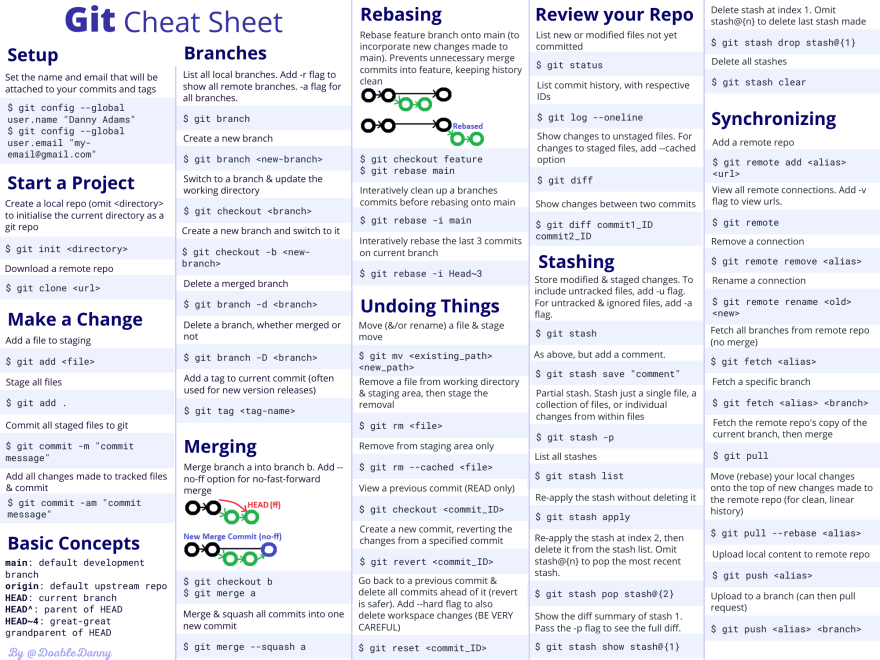
\includegraphics{Images/GitCheatSheet.png}
\caption{Git Cheat Sheet}
\end{figure}
\FloatBarrier
